\newpage
\section{Outlook}
The last section of this computing note focuses on the future of the CBM experiment. The first part describes different software components needed to operate the experiment with a focus on the \gls{DCS}. The second part illustrates potential upgrades and additions to the DCS in order to address components needed for a more complex system.
\subsection{Experiment controls architecture}
Figure \ref{fig_sim} depicts the targeted controls architecture of the future CBM experiment. According to CBM computing Note 18003 \cite{CBM_definitions} detector control and Interlock control are denoted as Experiment and Detector controls work packages 1 and 2. The respective control systems of the \gls{mCBM} experiment have been running in a standalone mode so far, which means that there hasn't been any structured communication between DCS, Device Control Agent (\gls{DCA}), and Experiment Control System (\gls{ECS}).

\begin{figure}[h!]
\centering
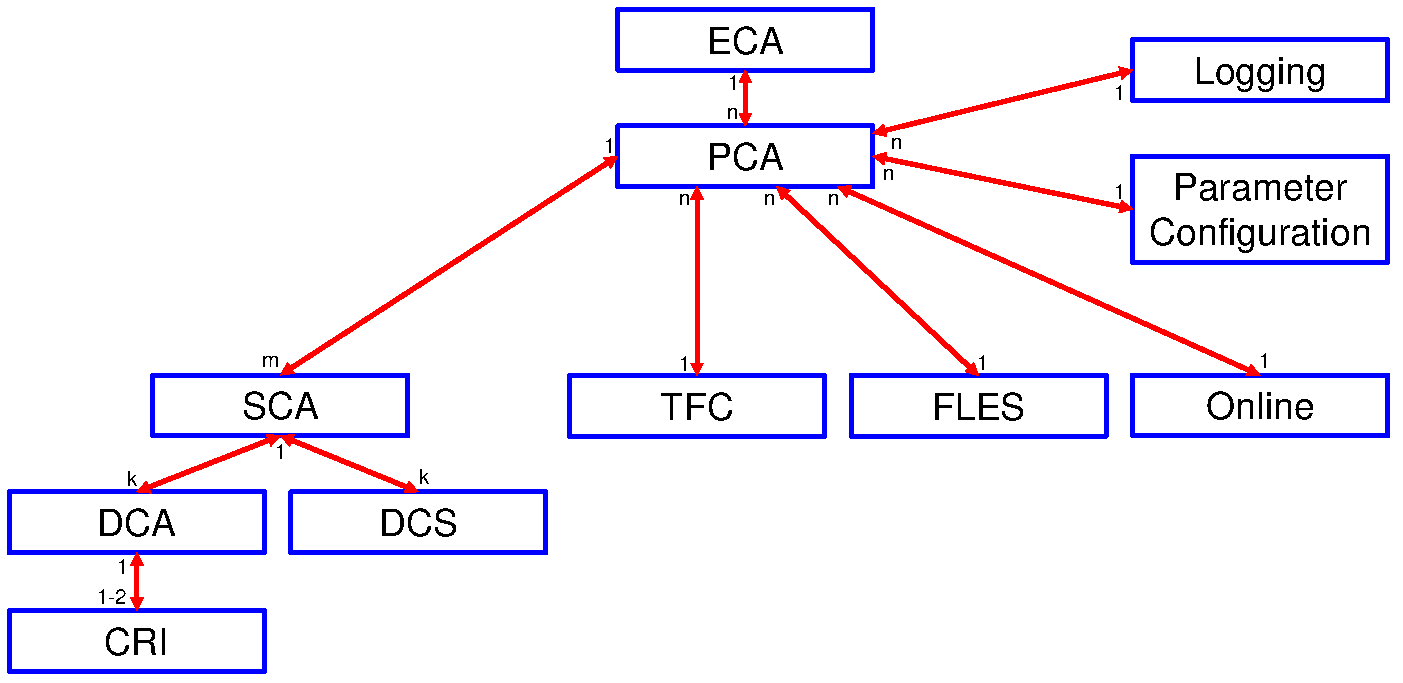
\includegraphics[width=0.8\columnwidth]{Chapter6/DCS/images/AgentsRelations_V2.pdf}
\caption{ECS core agent relations}
\label{fig_sim}
\end{figure}

\subsection{Experiment Control System (ESC)}\label{sssAgents}
The ECS consists of so-called software agents, which should efficiently manage all the subsystems in order to acquire data for the physics analysis.
The Experiment Control Agent, or ECA, is the top layer of the ECS core, which should be always running and keep track of 
the partitions, of the systems in partitions, and of the systems out of partitions.  It also manages the states of ``Central systems'' not having partition-level states (e.g., \gls{TFC}, FLESnet in case it does 
not use internal partitions). It provides upon request from agents the address and port needed to establish the 0MQ sockets and for building the 
ECS structure. The Partition Control Agent(s), or \gls{PCA}, is the bottom layer of the ECS, which track the state and controls a set of 
detector systems plus all needed central systems. It corresponds to the run context entity.  Any data run corresponds to a single partition. 
Multiple partitions can operate in parallel, potentially allowing to run~/~write parallel runs with independent 
detector system sets. 

The \glspl{PCA} also hold internal instances of the necessary SCA interfaces, which are tasked with:
\begin{itemize}
 \item holding a copy of the current state of the SCA
 \item periodic ping of the SCA to ensure early disconnection detection
 \item sending requests to the SCA and receiving the replies
 \item Monitoring the SCA broadcast channel for unexpected~/~unrequested state changes
\end{itemize}
These should not be confused with the SCA, which are in separate processes.

The following central SCA interfaces are expected:
\begin{itemize}
 \item Time and Fast Control (TFC)
 \item Accelerator signals (read-only)
 \item Interlock system (read-only)
 \item First Level Event Selector network (FLESnet)
 \item Online Event Selection, eventually linked to an Online Farm SCA
 \item Online Data QA a.k.a. Online Monitoring, eventually linked to an Online Farm SCA
 \item Setup description Management
 \item Configuration Management
 \item Logging storage system
 \item Monitoring storage system
\end{itemize}
The following detector SCA interfaces are expected (indicative, list will be dynamic and generic at PCA level):
\begin{itemize}
 \item Time zero (T0) a.k.a. Start Detector or Beam Monitor (BMON)
 \item Micro-Vertex Detector (MVD)
 \item Silicon Tracking System (STS)
 \item Ring Imaging CHerenkov (RICH)
 \item MUon CHambers (MUCH)
 \item Transition Radiation Detector (TRD)
 \item Time Of Flight wall (TOF)
 \item Beam Fragment Timing Counter (BFTC)
 \item Projectile Spectators Detector (PSD)
\end{itemize}
The subsystem-specific SCA should manage communication both with the DAQ chain and DCS. 
\subsection{Detector Control System (DCS)}
The mSTS didn't publish its overall status to any external agent. Due to that reason, some information like \gls{ASIC} internal temperature or $V_{DDM}$ were only accessible via the data acquisition chain (\gls{DCA}-\gls{CRI}). In the future, each subsystem will have an assigned \gls{SCA} to tackle control of the readout chain and the DCS. After almost two years of operation of the containers based \gls{DCS}, it proved to be a reliable, easily maintained solution. In addition to the existing system several additional applications are needed for the final system. The STS will be much more complex and challenging when it comes to configuration and running. Moreover, it will be extremely important to have both hardware and software interlocking to ensure the machine's safety.
Figure \ref{fig_arch} shows a general idea behind the STS's DCS from the software point of view. The master node or the central DCS node will get the data from the configuration database, which will allow to prepare subsystems for a given action (for example for a transition into a different state). Moreover, the master node will be only accessible by the DCS experts, excluding subsystem-related personnel from performing actions on other subsystems' DCS. 

\begin{figure}[!h]
\centering
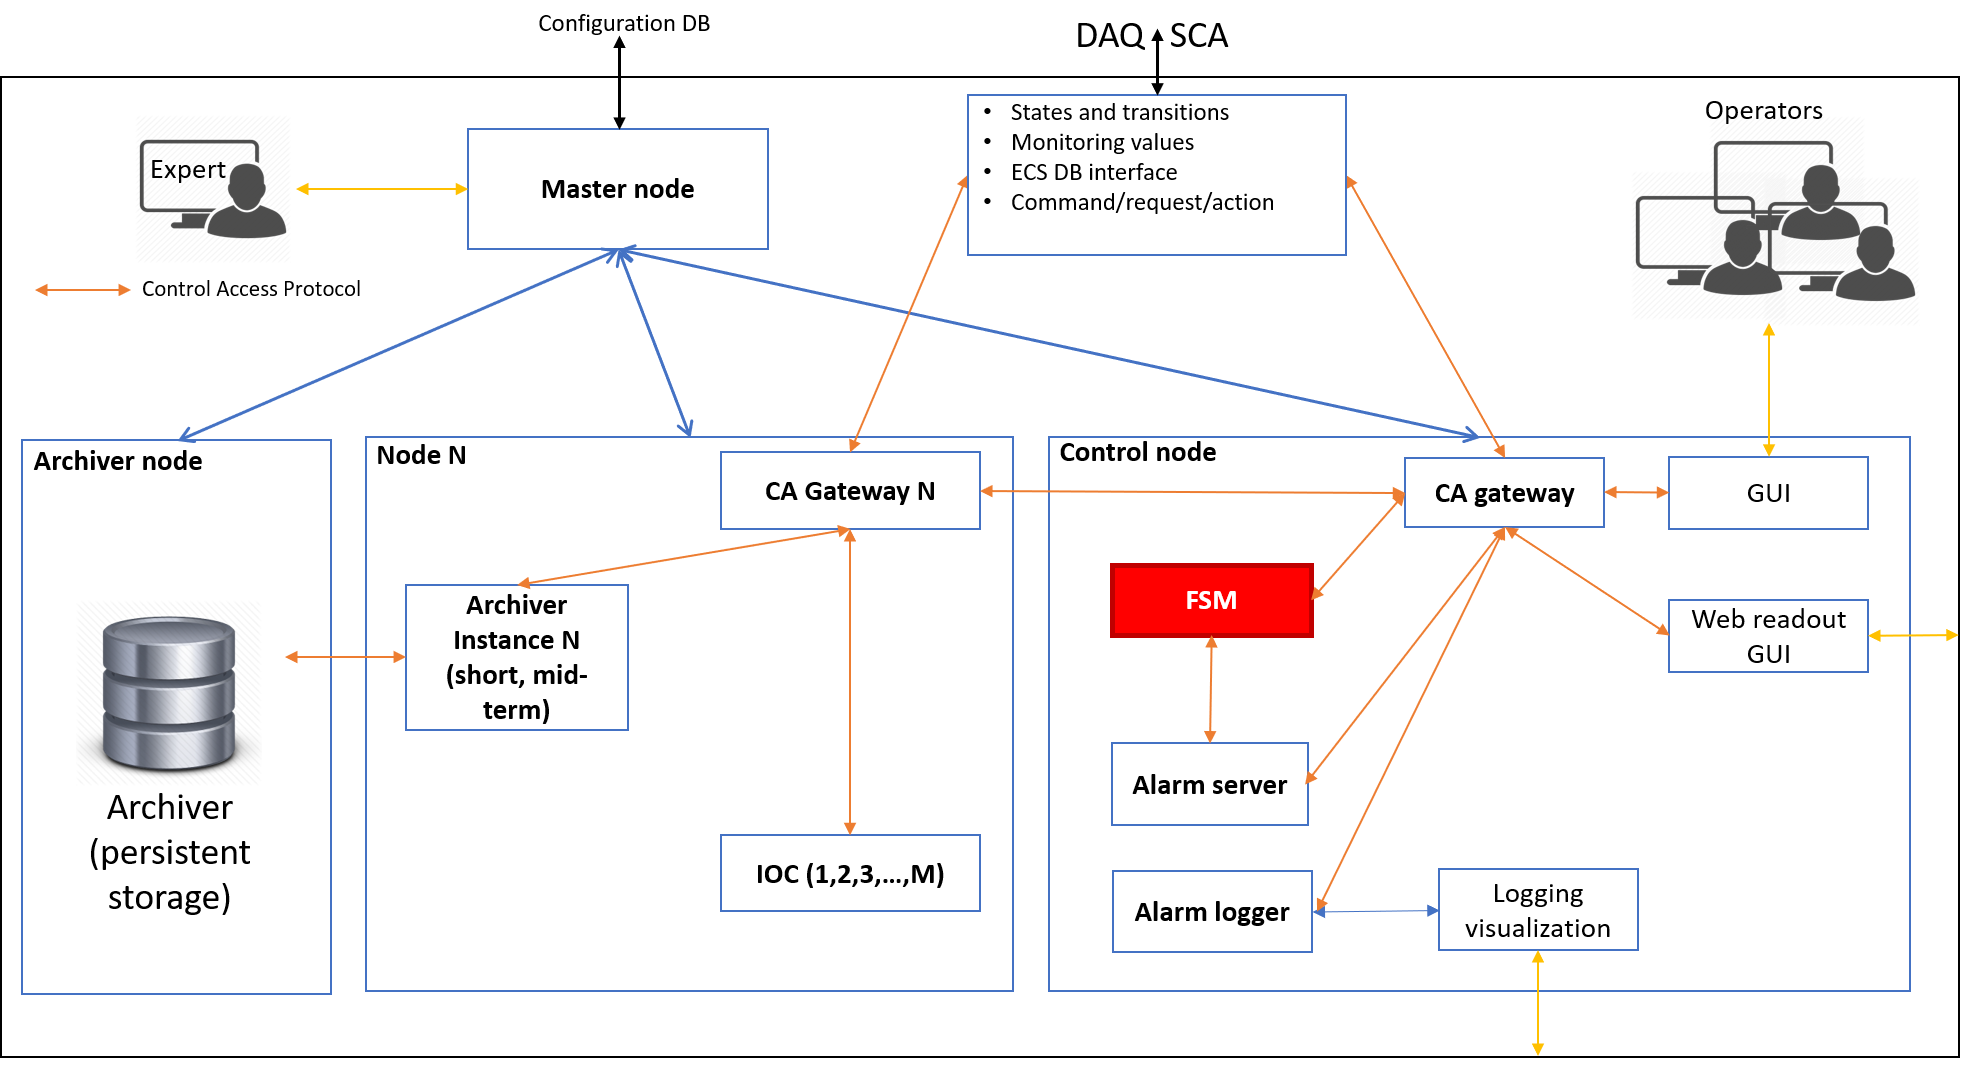
\includegraphics[width=0.85\columnwidth]{Chapter6/DCS/images/DCS.png}
\caption{Proposed DCS infrastructure for the STS}
\label{fig_arch}
\end{figure}
%\newpage
\subsection{Means of orchestration and maintenance} 
Weavescope provides basic monitoring and handling functionalities. Container metrics proved to be extremely useful in detecting issues and managing containers. For the final experiment, a much more sophisticated infrastructure is foreseen. Therefore, it's necessary to address it by automating deployment and monitoring. Similarly, as for the containers, an orchestrator needs to be secure, scalable, highly available, provide logging, monitoring capabilities, and be redundant. Orchestration leads to automation of the container deployment, as well as to balance the workload. 
Examples of orchestrators include DockerSwarm \cite{DockerSwarm}, and Kubernetes \cite{Kubernetes}. One of the recent applications of the Kubernetes was reported in \cite{ICALEPCS2021:Diamond}, where the whole test beamline is operated with containers. Similarly, the whole CBM's DCS will be operated with containers and orchestration tools. 
With container orchestration, it is possible to manage the lifecycle of applications or ecosystems of applications consisting of large numbers of containers. 

Orchestrators can:
 \begin{itemize}
     \item automatically deploy containers based on policies, application load, and environment metrics,
     \item identify failed containers or clusters and heal them,
     \item manage application configuration,
     \item connect containers to storage and manage networking,
     \item improve security by restricting access in between containers, and between containers and external systems.
 \end{itemize}
\subsection{Logbook}
One of the missing components in the mSTS's architecture is the logbook and the connection to it. The mSTS's environment is considered to be a development scene, therefore for the CBM experiment, a proper production environment has to be prepared. So far, for all mCBM-related activities, elog \cite{elog} was used. For the final experiment, a dedicated elog branch will be implemented and the elog client will be used \cite{elog_client}.
\subsection{Save and restore}
Save and restore functions can be divided into two groups of mechanisms. The first tool which provides save mechanisms is the so-called autosave, which is a part of the synApps module \cite{autosave}. It provides tools to preserve PVs values through an IOC reboot. The second set of tools that permits taking snapshots and saving configurations is MASAR \cite{masar}. It's a more complex tool than autosave, offering also a Phoebus-based \gls{GUI}. 
\subsection{Timing}
To properly archive and analyze the data, it's necessary that all nodes, \gls{IOC}s, and other software applications are synchronized. As it's impossible to adjust the clock in the containers, it should be synchronized on each node separately. The central \gls{DCS} node will provide a Network Time Protocol (\gls{NTP}) daemon that will be synchronized with one of the public, official sources.  By doing so, the clocks of all the containers running control applications will be automatically synchronized even if the external network connection is not available. 
\subsection{Failover considerations}
The high availability of services plays a key role in the safe operation of a detector. Once all the services are deployed, only minimal operation breaks are foreseen during 10 years of operation. The STS needs to be constantly cooled, in order to avoid performance degradation of the silicon sensors.
Crucial elements of the STS, like the air drying plant or the cooling plant, will be monitored and controlled by a PLC-based system (for example Siemens PLC). This hardware layer will provide the essential safety measures in case of failure but the PLC will be also linked to an IOC publishing the values to the software layer. Even before triggering the hardware interlock, any potentially hazardous system behavior will be discovered by the software of the control system. In order to ensure maximum safety, failover mechanisms will be exercised to mitiage potential IOC failures. There are 3 considered methods to address failover. 


If the hardware is controlled e.g., via a network, then it is possible to deploy a backup IOC, which has the same configuration as the main IOC, therefore providing a replacement if it fails. Nevertheless, under some standards like for example RS232, it is not considered good practice to have two \glspl{IOC} connected to the same node. Furthermore, in the case of RS232 a multiplexer would be needed to implement a redundant solution. 

A second possibility is to use failover mechanisms based on an orchestrator, in this case, the deployment and life-cycle of a container is governed by an additional tool, i.e., Kubernetes. In case one of the containers (IOCs) hangs up, it will be automatically stopped and a new container will take over the tasks. Nevertheless, the newly deployed container could have a different configuration, therefore changing the state of the whole system. 


\subsection{Data persistence}

As mentioned in the section \ref{archiver}, the archiver could be split into a few nodes serving as temporary data storage (short-term, mid-term). Proper daily backup to GSI managed database would be recommended, as it depends mostly on the database services provided by the GSI IT. So far, the Redis DB has been used but also other options should be considered. 

\subsection{Available protocols}
As reported during the EPICS Collaboration meeting 2022 \cite{epics_2022}, a transition to the newer protocol (PV access) is ongoing. Nevertheless, CA and PVA are both included in the EPICS 7, which should be the base image of the CBM IOC image, also for the next versions of the IOC. PVA is under constant development and will offer even more features in the coming years, thus for the future CBM experiment (timeline of more than 10 years) it is a perfect choice. 

\subsection{Use of gateways}
Lets consider the low voltage powering of the \gls{STS} \gls{FEE}, which consists of about 2100 low voltage channels, 140 modules, and 14 crates. Each crate has a controller with an embedded \gls{IOC}, publishing all the process variables. By putting the power supplies into a different subnet, we can not only easily debug potential issues but also limit the network traffic. That is why it has been endorsed to use CA Gateway \cite{gateway} or PV gateway (to be tested), which will take care of regulating access between the subnets in the DCS network. It also provides additional access security, assuring that the \glspl{IOC} running the key services like powering run smoothly.

